\section*{Ludwing Boltzmann\protect\footnote{\url{https://en.wikipedia.org/wiki/Ludwig_Boltzmann}}}

\begin{figure}[ht]
  \centering
  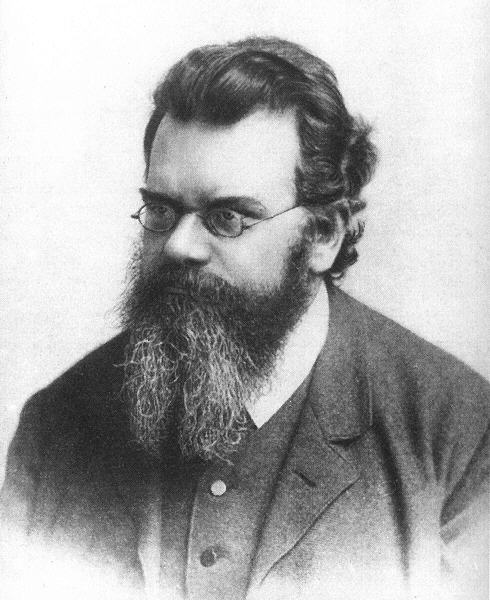
\includegraphics[width=0.8\linewidth]{content/figures/Boltzmann_figure.jpg}
  \caption{Albert Einstein in 1921\protect\footnotemark}
\end{figure}
\footnotetext{\url{https://upload.wikimedia.org/wikipedia/commons/a/ad/Boltzmann2.jpg}}

Boltzmann was born in Vienna, the capital of the Austrian Empire. His father, Ludwig Georg Boltzmann, was a revenue official. His grandfather, who had moved to Vienna from Berlin, was a clock manufacturer, and Boltzmann's mother, Katharina Pauernfeind, was originally from Salzburg. He received his primary education from a private tutor at the home of his parents. Boltzmann attended high school in Linz, Upper Austria. When Boltzmann was 15, his father died.

Boltzmann studied physics at the University of Vienna, starting in 1863. Among his teachers were Josef Loschmidt, Joseph Stefan, Andreas von Ettingshausen and Jozef Petzval. Boltzmann received his PhD degree in 1866 working under the supervision of Stefan; his dissertation was on kinetic theory of gases. In 1867 he became a Privatdozent (lecturer). After obtaining his doctorate degree, Boltzmann worked two more years as Stefan's assistant. It was Stefan who introduced Boltzmann to Maxwell's work.

In 1869 at age 25, thanks to a letter of recommendation written by Stefan,[2] he was appointed full Professor of Mathematical Physics at the University of Graz in the province of Styria. In 1869 he spent several months in Heidelberg working with Robert Bunsen and Leo Königsberger and then in 1871 he was with Gustav Kirchhoff and Hermann von Helmholtz in Berlin. In 1873 Boltzmann joined the University of Vienna as Professor of Mathematics and there he stayed until 1876.

In 1872, long before women were admitted to Austrian universities, he met Henriette von Aigentler, an aspiring teacher of mathematics and physics in Graz. She was refused permission to audit lectures unofficially. Boltzmann advised her to appeal, which she did, successfully. On July 17, 1876 Ludwig Boltzmann married Henriette; they had three daughters and two sons. Boltzmann went back to Graz to take up the chair of Experimental Physics. Among his students in Graz were Svante Arrhenius and Walther Nernst.[3][4] He spent 14 happy years in Graz and it was there that he developed his statistical concept of nature.

Boltzmann was appointed to the Chair of Theoretical Physics at the University of Munich in Bavaria, Germany in 1890. In 1893, Boltzmann succeeded his teacher Joseph Stefan as Professor of Theoretical Physics at the University of Vienna.

Boltzmann spent a great deal of effort in his final years defending his theories. He did not get along with some of his colleagues in Vienna, particularly Ernst Mach, who became a professor of philosophy and history of sciences in 1895. That same year Georg Helm and Wilhelm Ostwald presented their position on Energetics at a meeting in Lübeck. They saw energy, and not matter, as the chief component of the universe. Boltzmann's position carried the day among other physicists who supported his atomic theories in the debate.[5] In 1900, Boltzmann went to the University of Leipzig, on the invitation of Wilhelm Ostwald.[6] After the retirement of Mach due to bad health, Boltzmann returned to Vienna in 1902.[7] In 1903 he founded the Austrian Mathematical Society together with Gustav von Escherich and Emil Müller. His students included Karl Przibram, Paul Ehrenfest and Lise Meitner.

In Vienna, Boltzmann taught physics and also lectured on philosophy. Boltzmann's lectures on natural philosophy were very popular and received considerable attention. His first lecture was an enormous success. Even though the largest lecture hall had been chosen for it, the people stood all the way down the staircase. Because of the great successes of Boltzmann's philosophical lectures, the Emperor invited him for a reception at the Palace.

On September 5, 1906, while on a summer vacation in Duino, near Trieste, Boltzmann hanged himself.[8][9] He is buried in the Viennese Zentralfriedhof; his tombstone bears the inscription of the entropy formula:
\begin{equation}
	S=k\cdot \log W\,
\end{equation}
